\section{\textit{Retrieval Augmented Generation} (RAG)} % Seções são adicionadas para organizar sua apresentação em blocos discretos, todas as seções e subseções são automaticamente exibidas no índice como uma visão geral da apresentação, mas NÃO são exibidas como slides separados.
%----------------------------------------------------------------------------------------
\begin{frame}
	\frametitle{\textit{Retrieval Augmented Generation} (RAG)}
	{\footnotesize
		\begin{itemize}
			\item RAG é uma técnica que combina  LLMs com sistemas de \textbf{recuperação de informação }
			\item  A recuperação de informação (\textit{retrieval}) realiza uma busca dos \textbf{documentos pertinentes} à \textit{query} de modo que eles sejam combinados para formar o \textit{input} do LLM
			\item Fixado o LLM utilizado no sistema, a pertinência dos documentos à \textit{query} está diretamente relacionada à qualidade do \textit{output} gerado pelo RAG
		\end{itemize}
	}
	\begin{figure}[H]
		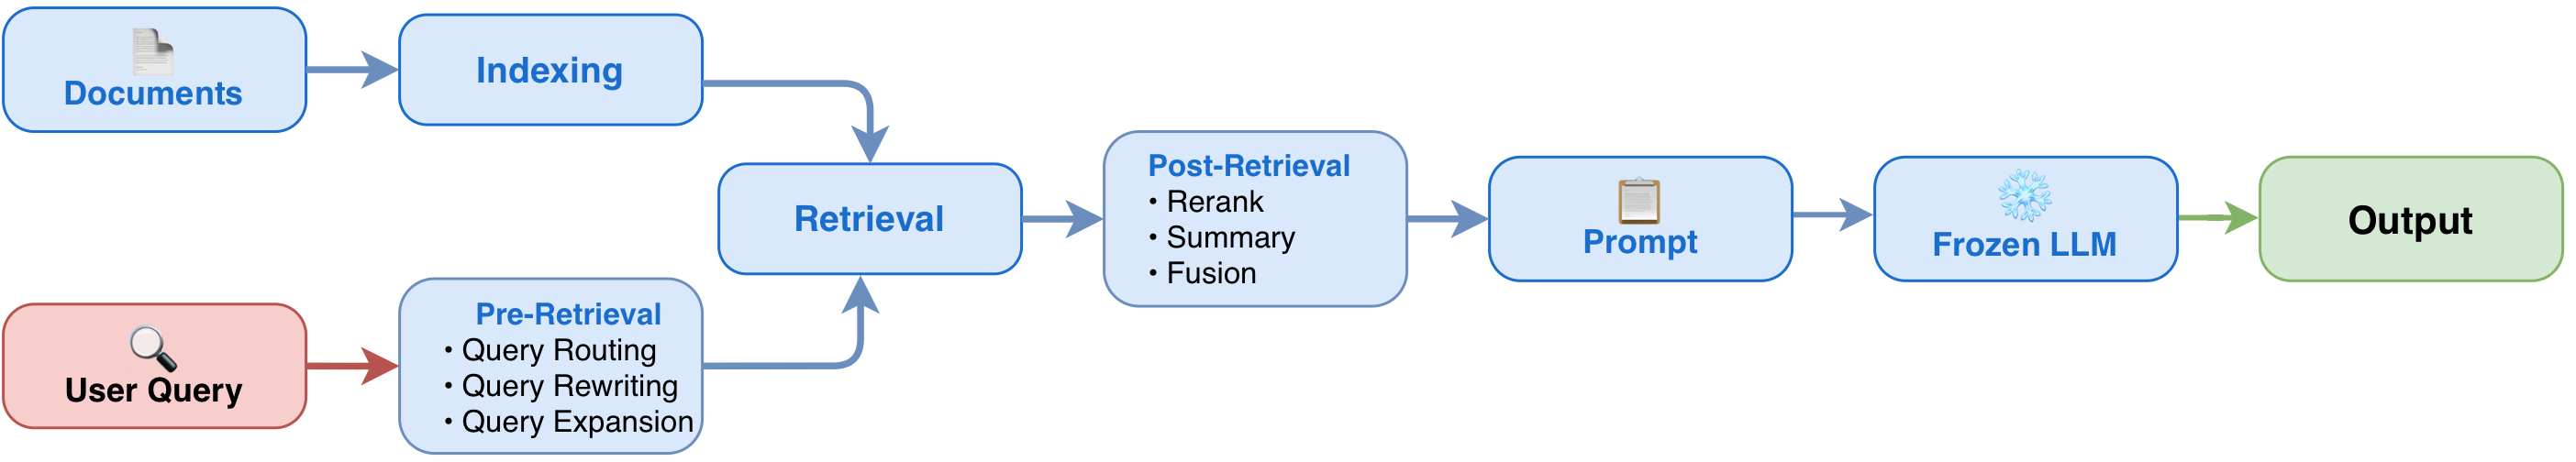
\includegraphics[width=0.85\linewidth]{img/rag_arch.png}
	\end{figure}
\end{frame}
%----------------------------------------------------------------------------------------
\begin{frame}
	\frametitle{Seleção de Documentos Pertinentes}
	\begin{columns}
		\begin{column}{0.50\textwidth}
			{\footnotesize
				\begin{itemize}
					\item A escolha de documentos relevantes à \textit{query} é de responsabilidade da etapa de busca
					\item A \textbf{similaridade de cosseno} é a técnica comumente utilizada para definir relevância
					\item O mesmo modelo de \textit{embeddings} utilizado para gerar os vetores dos \textit{chunks} é utilizado para gerar um vetor da \textit{query}, o que habilita o sistema a utilizar o produto interno entre \textit{chunks} e \textit{query}
				\end{itemize} 
			}
		\end{column}
		\begin{column}{0.40\textwidth}
			\begin{figure}[H]
				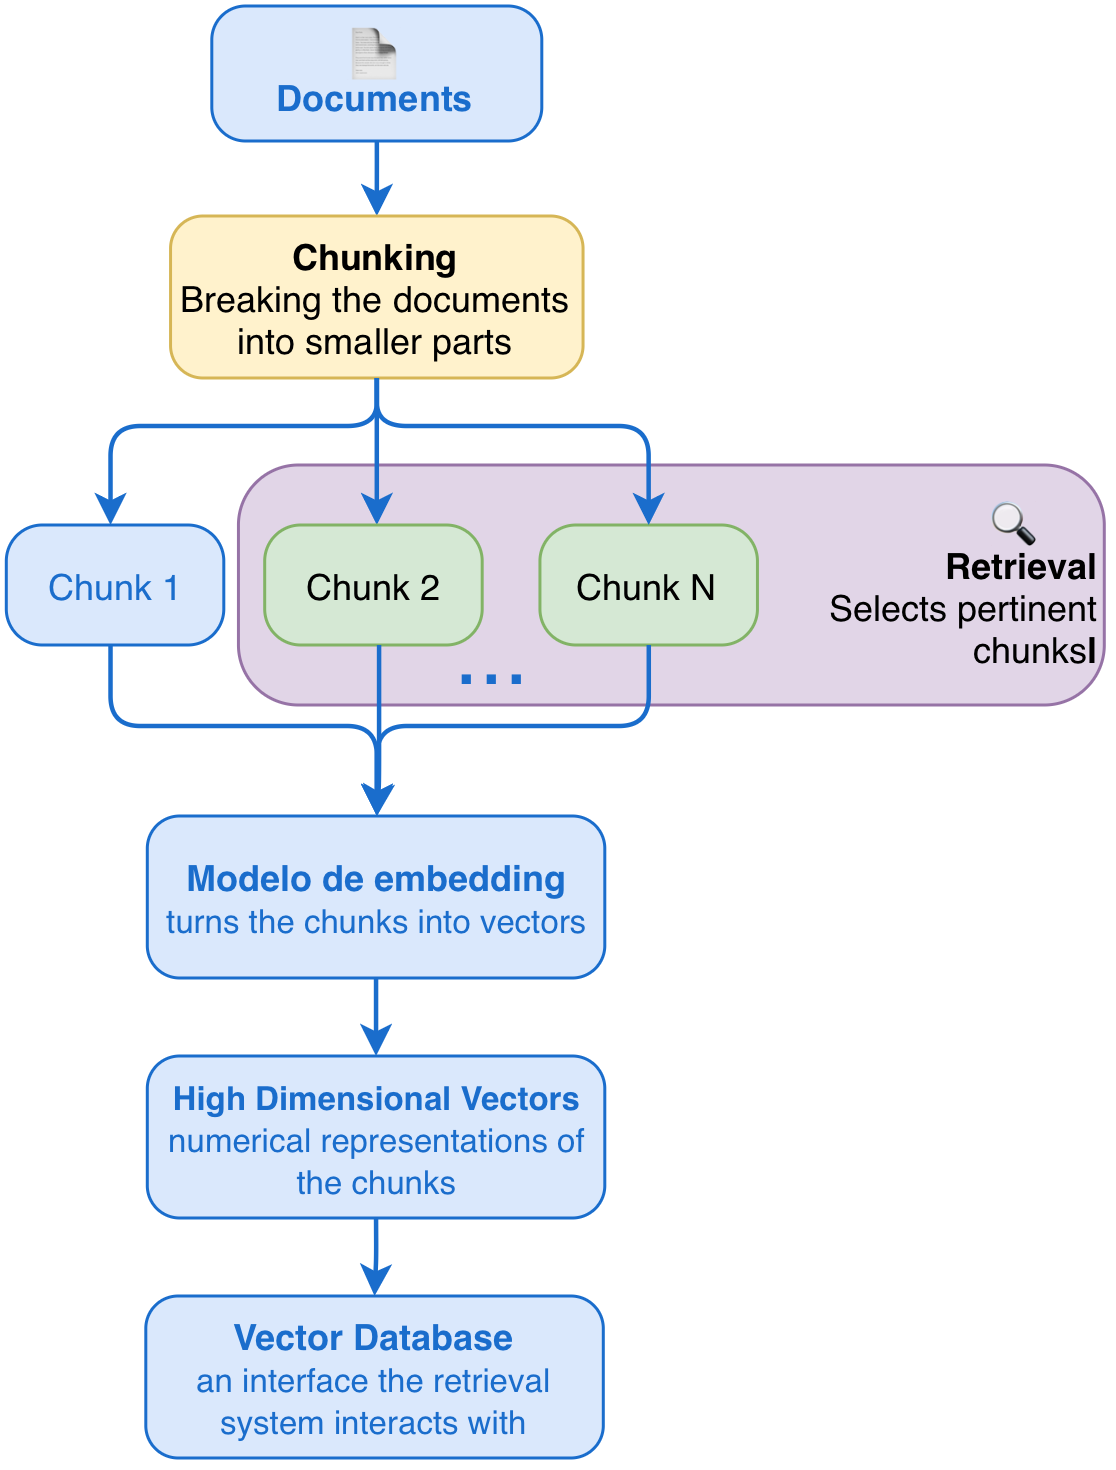
\includegraphics[width=\linewidth]{img/pertinent_chunks_selection.png}
			\end{figure}
		\end{column}
	\end{columns}
\end{frame}
%----------------------------------------------------------------------------------------
\begin{frame}
	\frametitle{Problemas com a Busca Vetorial Pura}
	{\footnotesize
		\begin{itemize}
			\item Seleção de documentos irrelevantes à \textit{query}
			\item Seleção de documentos contraditórios ao conhecimento de domínio
			\item Menor correção atribuída aos \textit{outputs} gerados pelo LLM
			\item Baixa explicabilidade
		\end{itemize}
	}
	
	\begin{figure}[H]
		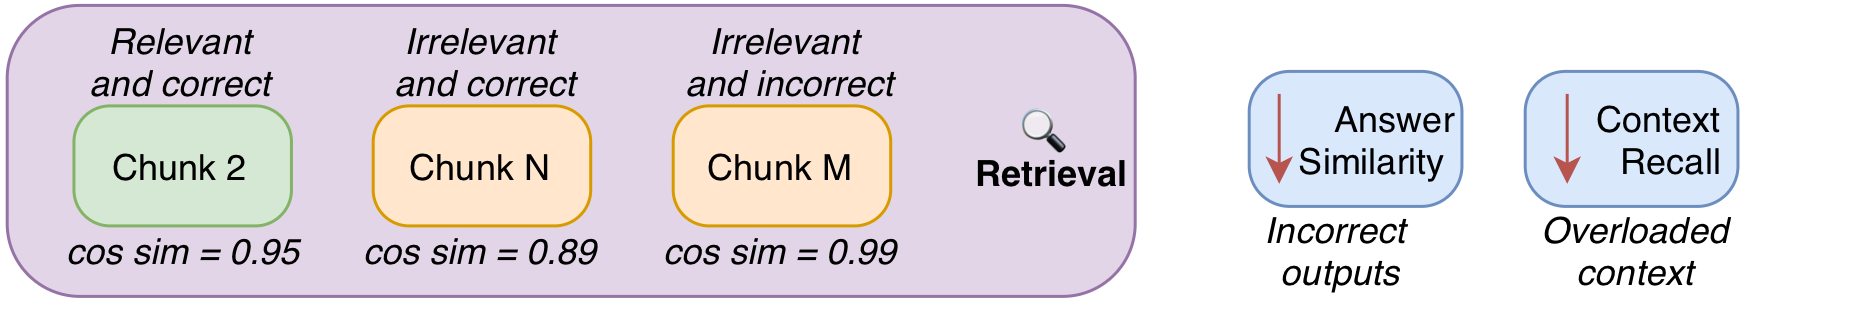
\includegraphics[width=0.85\linewidth]{img/cos_sim_problems.png}
	\end{figure}
	
\end{frame}
%---------------

%----------------------------------------------------------------------------------------